\subsection{Two Fixed Batches Under a Random Common Stretch}
\label{sec:stretch-experiment}

We finally check the executable upper-bound construction on a template
with two batches of two candidates, $\boldsymbol\alpha=(4,1)$ and $K=5$.
Let $T=4\cdot4^m$, $m=3,4,5,6$, and let $H$ range over
$1,4,\ldots,4^m$.  We consider the inverse-square-root law
$\PP(H=4^j)\propto2^{-j}$, the uniform law on these scales, and the
deterministic longest scale.  Once the first batch arrives, the rule in
Theorem~\ref{thm:random-positive-main} runs fresh fixed-horizon MOSS experiments
of lengths $3H$ and $H$.  The comparison is the original anytime MC-MOSS,
which retains all observations, including the anchor's prefix.  The
former rule uses the known endpoint and revealed schedule; MC-MOSS is
given neither.

The fixed reward vector is
$(0.50,0.45,0.55,0.55+\eta\delta,0.50)$, with
$\eta\in\{-1,1\}$ and
$\delta\in\{0.025,0.05,0.10,0.20,0.40\}$.
For each $(m,Q)$ we use 64 development replications to select the single
pair $(\eta,\delta)$ with the largest law-averaged regret for the
revealed-stretch rule.  We evaluate that same pair on 128 independent
held-out replications for both policies and every value of $H$.
Thus no environment is selected after the realized stretch.  The finite
law is averaged exactly over its support, with Monte Carlo sampling only
for rewards.  These are held-out risks for selected common environments,
not estimates of the continuous minimax supremum.



At $m=6$, the inverse-square-root law has $W(Q)=1.386$;
the revealed-stretch rule has mean regret $5.94$ (standard error $0.05$),
and MC-MOSS has $3.11$ ($0.06$).  The corresponding revealed-stretch risks
are $39.81$ ($0.58$) under the uniform-scale law and $141.80$ ($3.14$)
under the deterministic longest scale, whose complexities are $12.190$
and $64$, respectively.  Figure~\ref{fig:stretch-heldout} displays the
normalized values across all four endpoints.  MC-MOSS performs better
in every selected cell, despite using less schedule information.  This
does not contradict the theorem: the reset construction proves an
upper bound and is not optimized for finite-sample constants.  Nor does
this finite grid establish the asymptotic rate or a matching lower
constant.  Its role is to verify that the common-environment averaging
and the multi-batch upper-bound rule can be implemented without
discarding regret incurred before the last batch.


\begin{figure}[tbp]
\centering
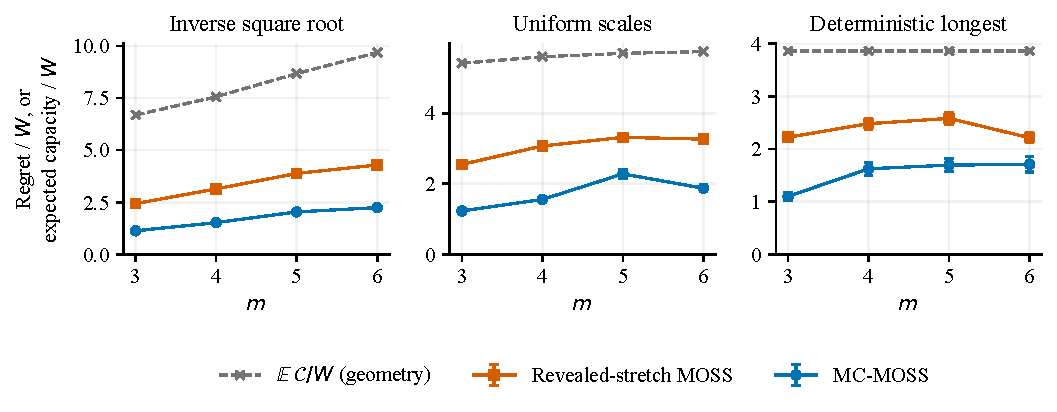
\includegraphics[width=\linewidth]{figures_v2/fig_stretch_heldout.pdf}
\caption{Held-out common-environment risks divided by $W(Q)$ for the
fixed two-batch template.  Error bars are $1.96$ Monte Carlo standard
errors under exact stratification over $H$.  The dashed curve is the
expected deterministic capacity divided by $W(Q)$ and is a geometric
reference, not an observed regret.  Both policies face the same
development-selected environment in each panel and at each $m$.}
\label{fig:stretch-heldout}
\end{figure}